\chapter{État de l'Art et Spécification des Besoins}

\section{Introduction}

L'analyse sportive assistée par l'intelligence artificielle connaît une croissance exponentielle ces dernières années. Ce chapitre explore l'état de l'art des technologies et systèmes existants dans le domaine du sport analytics, avant de définir les besoins spécifiques auxquels notre solution SmartClub Analytics doit répondre.

\section{État de l'Art des Systèmes d'Analyse Sportive}

\subsection{Plateformes Commerciales Existantes}

Le marché du sport analytics est dominé par plusieurs plateformes professionnelles :

\begin{itemize}
    \item \textbf{Catapult Sports} : Système de tracking GPS et analyse de charge d'entraînement utilisé par les équipes professionnelles. Propose des métriques de performance et de risque de blessure, mais reste très coûteux et nécessite un hardware propriétaire.
    
    \item \textbf{Zone7} : Plateforme IA spécialisée dans la prédiction de blessures chez les athlètes. Utilise des modèles de deep learning sur des données biomécaniques et physiologiques. Offre une précision remarquable mais son intégration est complexe et son coût d'abonnement élevé.
    
    \item \textbf{Kinexon} : Solution de tracking en temps réel avec capteurs UWB. Fournit des données de position, vitesse, accélération et charge de travail. Principalement utilisé dans les sports d'équipe professionnels.
    
    \item \textbf{StatsBomb} : Plateforme d'analyse de données de football avec des métriques avancées comme les expected goals (xG) et expected assists (xA). Excellente pour l'analyse de performance mais ne couvre pas la prévention des blessures.
\end{itemize}

\subsection{Limitations des Solutions Existantes}

\begin{itemize}
    \item \textbf{Coût prohibitif} : La plupart des solutions professionnelles nécessitent des budgets importants, les rendant inaccessibles aux clubs amateurs et semi-professionnels.
    \item \textbf{Complexité technique} : L'intégration de ces systèmes requiert une expertise technique que peu de clubs possèdent en interne.
    \item \textbf{Manque de personnalisation} : Ces plateformes sont souvent conçues pour des besoins génériques et ne s'adaptent pas aux spécificités de chaque club.
    \item \textbf{Modules disjoints} : Les clubs doivent souvent utiliser plusieurs solutions distinctes pour la nutrition, la physiothérapie, le scouting et la gestion des contrats.
\end{itemize}

\subsection{Avancées en IA pour le Sport}

\subsubsection{Prédiction de Blessures}

La recherche académique a démontré plusieurs approches prometteuses :

\begin{itemize}
    \item \textbf{Modèles de séries temporelles} : L'utilisation de LSTM (Long Short-Term Memory) sur les données de charge d'entraînement permet de prédire les fenêtres de risque accru de blessure avec une précision de 75-85\% \cite{bienefeld2023}.
    
    \item \textbf{ACWR (Acute:Chronic Workload Ratio)} : Métrique standardisée qui compare la charge de travail aiguë (7 jours) à la charge chronique (28 jours). Un ratio entre 0.8 et 1.3 est considéré optimal, tandis que des valeurs supérieures à 1.5 indiquent un risque significatif de blessure \cite{gabbett2016}.
    
    \item \textbf{Random Forests et Gradient Boosting} : Des études récentes montrent que ces algorithmes d'ensemble atteignent une AUC de 0.82-0.88 pour la classification du risque de blessure en utilisant des caractéristiques combinées de charge, de fatigue, et d'historique médical.
\end{itemize}

\subsubsection{Traitement du Langage Naturel pour le Coaching}

Les LLMs (Large Language Models) comme ceux disponibles via l'API Groq ou OpenAI ouvrent de nouvelles possibilités :

\begin{itemize}
    \item \textbf{Analyse conversationnelle} : Permettre aux entraîneurs d'interroger les données sportives en langage naturel.
    \item \textbf{Génération de rapports} : Production automatisée de rapports d'analyse après chaque match ou session d'entraînement.
    \item \textbf{Support multilingue} : Capacité à interagir dans différentes langues (français, anglais, arabe, tunisien) pour s'adapter aux utilisateurs locaux.
\end{itemize}

\subsubsection{Systèmes de Recommandation Nutritionnelle}

L'intégration de bases de données nutritionnelles (telles que FoodData Central de l'USDA) avec des modèles de planification alimentaire permet de générer des plans nutritionnels personnalisés en fonction des objectifs de performance et de récupération des athlètes.

\section{Analyse des Besoins}

\subsection{Besoins Fonctionnels}

L'analyse des besoins a été réalisée en collaboration avec des entraîneurs, des préparateurs physiques et des gestionnaires de clubs sportifs tunisiens.

\subsubsection{Module de Physiothérapie et Prévention des Blessures}

\begin{itemize}
    \item \textbf{BF-01} : Calcul et visualisation de l'ACWR pour chaque joueur.
    \item \textbf{BF-02} : Détection précoce des joueurs à risque de blessure.
    \item \textbf{BF-03} : Recommandations personnalisées de charge d'entraînement.
    \item \textbf{BF-04} : Tableau de bord quotidien des risques de l'effectif.
    \item \textbf{BF-05} : Suivi de l'évolution temporelle des métriques de performance.
\end{itemize}

\subsubsection{Module Nutritionnel}

\begin{itemize}
    \item \textbf{BN-01} : Consultation d'une base de données alimentaires riche (nutriments, calories, macronutriments).
    \item \textbf{BN-02} : Génération de plans nutritionnels personnalisés selon l'intensité d'entraînement.
    \item \textbf{BN-03} : Calcul automatique des macros pour les repas.
    \item \textbf{BN-04} : Recherche d'aliments et de suppléments sportifs.
\end{itemize}

\subsubsection{Module de Scouting et Analyse de Performance}

\begin{itemize}
    \item \textbf{BS-01} : Exploration et filtrage de profils de joueurs.
    \item \textbf{BS-02} : Analyse comparative des performances (xG, xA, passes décisives).
    \item \textbf{BS-03} : Visualisation des métriques clés par poste.
    \item \textbf{BS-04} : Suivi des statistiques de buts et d'assists.
\end{itemize}

\subsubsection{Module Assistant IA Conversationnel}

\begin{itemize}
    \item \textbf{BA-01} : Interface de chat en langage naturel pour interroger toutes les données.
    \item \textbf{BA-02} : Support multilingue (français, anglais, arabe, dialecte tunisien).
    \item \textbf{BA-03} : Exécution d'outils spécialisés (risque de blessure, nutrition, scouting).
    \item \textbf{BA-04} : Streaming des réponses pour une expérience utilisateur fluide.
\end{itemize}

\subsection{Besoins Non-Fonctionnels}

\begin{itemize}
    \item \textbf{BNF-01 - Performance} : Temps de réponse inférieur à 2 secondes pour les requêtes standards, inférieur à 5 secondes pour les analyses complexes.
    \item \textbf{BNF-02 - Sécurité} : Authentification JWT, contrôle d'accès basé sur les rôles (RBAC), protection CSRF.
    \item \textbf{BNF-03 - Évolutivité} : Architecture modulaire permettant l'ajout de nouveaux modules sans impact sur l'existant.
    \item \textbf{BNF-04 - Disponibilité} : Taux de disponibilité de 99,5\% pour les fonctionnalités critiques.
    \item \textbf{BNF-05 - Portabilité} : Déploiement possible sur site (on-premise) ou dans le cloud.
    \item \textbf{BNF-06 - Maintenabilité} : Code documenté, tests automatisés, architecture en couches.
\end{itemize}

\subsection{Diagramme de Cas d'Utilisation}

\begin{figure}[H]
\centering
\begin{tikzpicture}[
    scale=0.85, transform shape,
    actor/.style={rectangle, draw, minimum width=2cm, minimum height=0.8cm, font=\small, rounded corners, fill=blue!10},
    usecase/.style={ellipse, draw, minimum width=2.5cm, minimum height=0.8cm, font=\small, fill=green!10}
]
% Acteurs
\node[actor] (coach) at (-4,4) {Entraîneur};
\node[actor] (physio) at (-4,1) {Physio};
\node[actor] (manager) at (-4,-2) {Manager};
\node[actor] (admin) at (-4,-4) {Admin};

% Système
\draw[thick] (-1,-5) rectangle (12,6);
\node at (5.5,5.5) {\textbf{SmartClub Analytics}};

% Cas d'utilisation - Physio
\node[usecase] (risk) at (2,3) {Consulter risques\\de blessure};
\node[usecase] (acwr) at (5,3) {Visualiser ACWR};
\node[usecase] (profiles) at (8,3) {Profils joueurs};
\node[usecase] (nutrition) at (2,0) {Plans nutritionnels};
\node[usecase] (food) at (5,0) {Base alimentaire};
\node[usecase] (scout) at (8,0) {Analyse\\scouting};
\node[usecase] (chat) at (5,-2) {Assistant IA\\conversationnel};
\node[usecase] (auth) at (2,-4) {Authentification};
\node[usecase] (adminuc) at (8,-4) {Gestion\\utilisateurs};

% Relations acteurs -> cas
\draw (coach) -- (risk);
\draw (coach) -- (acwr);
\draw (coach) -- (chat);
\draw (physio) -- (risk);
\draw (physio) -- (profiles);
\draw (physio) -- (nutrition);
\draw (manager) -- (scout);
\draw (manager) -- (food);
\draw (manager) -- (nutrition);
\draw (admin) -- (auth);
\draw (admin) -- (adminuc);

% Relations include/extend
\draw[->,dashed] (risk) -- node[above,font=\tiny] {include} (acwr);
\draw[->,dashed] (nutrition) -- node[above,font=\tiny] {include} (food);

\end{tikzpicture}
\caption{Diagramme des cas d'utilisation du système SmartClub Analytics}
\label{fig:usecase}
\end{figure}

\section{Choix Technologiques}

\subsection{Backend : Django REST Framework}

Le choix de Django comme framework backend principal est motivé par :

\begin{itemize}
    \item \textbf{Robustesse et maturité} : Django est un framework éprouvé avec une communauté large et active.
    \item \textbf{ORM puissant} : L'Object-Relational Mapping de Django facilite l'interaction avec la base de données PostgreSQL.
    \item \textbf{Sécurité intégrée} : Protection CSRF, XSS, SQL injection, authentification JWT via SimpleJWT.
    \item \textbf{Django REST Framework} : Création rapide d'APIs RESTful avec sérialisation, validation et documentation automatique.
    \item \textbf{Écosystème riche} : Nombreuses extensions disponibles (caching, background tasks, etc.).
\end{itemize}

\subsection{Frontend : React avec Tailwind CSS}

\begin{itemize}
    \item \textbf{React 18} : Bibliothèque JavaScript moderne pour la création d'interfaces utilisateur réactives.
    \item \textbf{Tailwind CSS} : Framework CSS utilitaire permettant un développement rapide et cohérent.
    \item \textbf{Recharts} : Bibliothèque de visualisation de données pour les graphiques (ACWR, tendances, etc.).
    \item \textbf{Architecture modulaire} : Composants réutilisables et lazy-loading pour des performances optimales.
\end{itemize}

\subsection{Intelligence Artificielle : LLM et Machine Learning}

\begin{itemize}
    \item \textbf{API Groq} : Inférence LLM ultra-rapide pour l'assistant conversationnel (modèle Llama 3.1 8B).
    \item \textbf{Scikit-learn} : Implémentation des modèles de prédiction de blessures (Random Forest, Gradient Boosting).
    \item \textbf{FoodData Central} : Base de données nutritionnelle de l'USDA intégrée pour les recommandations alimentaires.
    \item \textbf{Modèles personnalisés} : Notebooks Jupyter pour l'entraînement de modèles de prédiction d'absence et de risque de blessure.
\end{itemize}

\subsection{Infrastructure : Docker et Conteneurisation}

\begin{itemize}
    \item \textbf{Docker Compose} : Orchestration des services (backend, frontend, base de données).
    \item \textbf{Nginx} : Serveur proxy inverse pour le routage et la gestion des requêtes.
    \item \textbf{PostgreSQL} : Base de données relationnelle robuste et performante.
\end{itemize}

\section{Architecture Globale du Système}

\subsection{Vue d'Ensemble}

L'architecture de SmartClub Analytics suit un modèle en couches :

\begin{figure}[H]
\centering
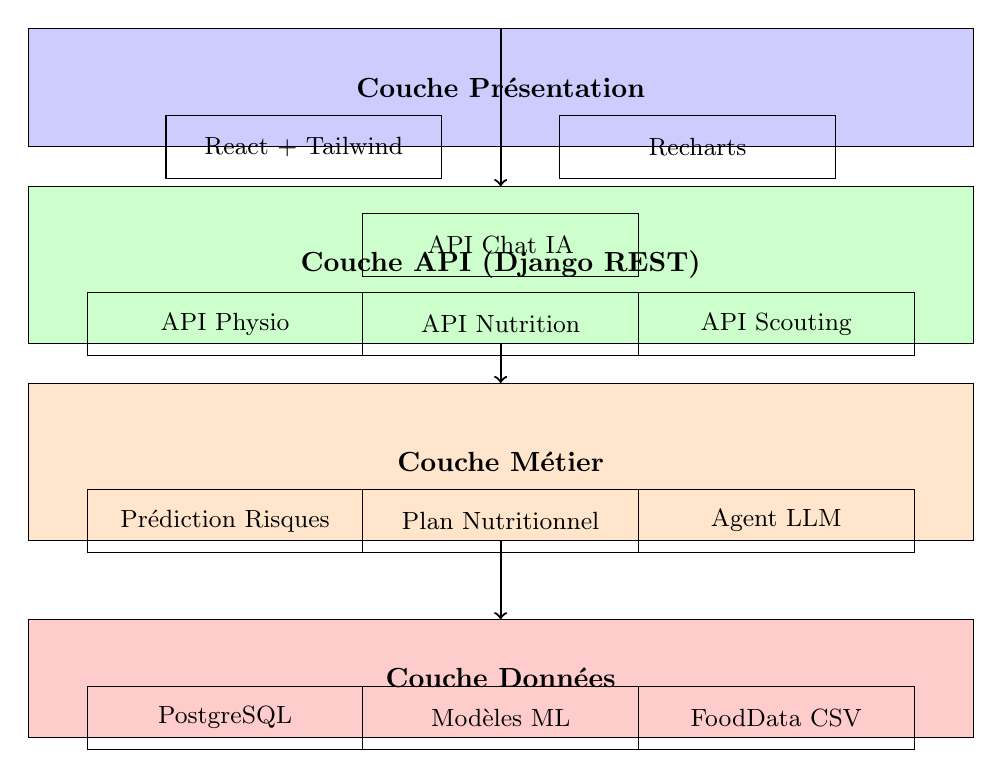
\begin{tikzpicture}[
    layer/.style={rectangle, rounded corners, minimum width=12cm, minimum height=1cm, text centered, font=\bfseries},
    comp/.style={rectangle, draw, minimum width=3.5cm, minimum height=0.8cm, font=\small}
]

% Couche Présentation
\draw[fill=blue!20] (-6,5) rectangle (6,6.5);
\node[layer] at (0,5.75) {Couche Présentation};
\node[comp] (react) at (-2.5,5) {React + Tailwind};
\node[comp] (charts) at (2.5,5) {Recharts};

% Couche API
\draw[fill=green!20] (-6,2.5) rectangle (6,4.5);
\node[layer] at (0,3.5) {Couche API (Django REST)};
\node[comp] (physioapi) at (-3.5,2.75) {API Physio};
\node[comp] (nutriapi) at (0,2.75) {API Nutrition};
\node[comp] (scoutapi) at (3.5,2.75) {API Scouting};
\node[comp] (chatai) at (0,3.75) {API Chat IA};

% Couche Métier
\draw[fill=orange!20] (-6,0) rectangle (6,2);
\node[layer] at (0,1) {Couche Métier};
\node[comp] (riskmod) at (-3.5,0.25) {Prédiction Risques};
\node[comp] (nutrimod) at (0,0.25) {Plan Nutritionnel};
\node[comp] (llmmod) at (3.5,0.25) {Agent LLM};

% Couche Données
\draw[fill=red!20] (-6,-2.5) rectangle (6,-1);
\node[layer] at (0,-1.75) {Couche Données};
\node[comp] (pg) at (-3.5,-2.25) {PostgreSQL};
\node[comp] (ml) at (0,-2.25) {Modèles ML};
\node[comp] (fooddb) at (3.5,-2.25) {FoodData CSV};

% Flèches
\draw[->,thick] (0,6.5) -- (0,4.5);
\draw[->,thick] (0,2.5) -- (0,2);
\draw[->,thick] (0,0) -- (0,-1);

\end{tikzpicture}
\caption{Architecture en couches de SmartClub Analytics}
\label{fig:architecture}
\end{figure}

\subsection{Flux de Données}

\begin{enumerate}
    \item L'utilisateur interagit via l'interface React ou le chatbot conversationnel.
    \item Les requêtes sont routées via le proxy Nginx vers les endpoints Django appropriés.
    \item Le backend traite la requête : interroge la base de données, exécute des modèles ML ou appelle l'API LLM.
    \item Les résultats sont sérialisés et renvoyés au frontend pour affichage.
    \item Pour l'assistant IA, un agent orchestrateur gère les appels d'outils (tool calling) en plusieurs itérations.
\end{enumerate}

\section{Conclusion}

Ce chapitre a présenté l'état de l'art des systèmes d'analyse sportive, identifié les lacunes des solutions existantes, et défini les besoins fonctionnels et non-fonctionnels de SmartClub Analytics. Les choix technologiques retenus (Django, React, LLM, Docker) répondent aux exigences de performance, sécurité et évolutivité du projet. Le chapitre suivant détaillera la conception du système à travers des diagrammes UML complets.

